\documentclass[11pt]{article}
\usepackage[top=1in, bottom=1in, left=1in, right=1in]{geometry}
\usepackage{tikz}
\usetikzlibrary{shapes,arrows,matrix,patterns,positioning}
\usepackage{color}
%\usepackage[parfill]{parskip}
\usepackage{graphicx}
\usepackage{algorithmic}
\usepackage{amssymb}
\usepackage{epstopdf}
\usepackage[ruled]{algorithm2e}
\usepackage{float}
\usepackage{amsmath,amsthm,bm,color,epsfig,enumerate,caption}
\usepackage{hyperref}
\usepackage{booktabs}
\usepackage{multirow}
\usepackage{array}

%\linespread{2}

% to highlight the latest changes
\newcommand{\alert}[1]{\textcolor{red}{#1}}

\newcommand{\hz}[1]{{\textbf{HZ: #1}}}
\newcommand{\yl}[1]{\textcolor{orange}{\textbf{Ryan: #1}}}
\newcommand{\erm}[1]{\textcolor{red}{\textbf{EM: #1}}}
\newtheorem{theorem}{Theorem}[section]
\newtheorem{outline}[theorem]{Outline}
\newtheorem{corollary}[theorem]{Corollary}
\newtheorem{definition}[theorem]{Definition}
\newtheorem{lemma}[theorem]{Lemma}
\newtheorem{proposition}[theorem]{Proposition}
\newtheorem{algo}[theorem]{Algorithm}
\newtheorem{remark}[theorem]{Remark}
\renewcommand{\appendix}[1]{
\section*{Appendix: #1}
}
\newcommand{\norm}[1]{\left\lVert#1\right\rVert}
%\newcommand{\herm}[1]{(#1)^*}
%\renewcommand{\L}{\mathcal{L}}
%\renewcommand{\O}{\mathcal{O}}
\renewcommand{\O}{O}
%\newcommand{\K}{\mathcal{K}}
%\newcommand{\F}{\mathcal{F}}
\newcommand{\bbZ}{\mathbb{Z}}
\newcommand{\bbF}{\mathbb{F}}
\newcommand{\bbC}{\mathbb{C}}
\newcommand{\bbR}{\mathbb{R}}
\newcommand{\rID}{{\it rID}}
\newcommand{\cID}{{\it cID}}
\newcommand{\blue}{\textcolor{blue}}

\makeatletter
\newcommand*{\extendadd}{
  \mathbin{
    \mathpalette\extend@add{}
  }
}
\newcommand*{\extend@add}[2]{
  \ooalign{
    $\m@th#1\leftrightarrow$%
    \vphantom{$\m@th#1\updownarrow$}
    \cr
    \hfil$\m@th#1\updownarrow$\hfil
  }
}
\makeatother

\begin{document}

\title{Numerical Comparison Summary}
%\author{Qiyuan Pang \\ Tsinghua University, China\\  \href{mailto:ppangqqyz@foxmail.com}{ppangqqyz@foxmail.com} 
%   \and Kenneth L. Ho \\ San Francisco, CA, USA\\ \href{mailto:klho@alumni.caltech.edu}{klho@alumni.caltech.edu}
%     \and Haizhao Yang \\ Department of Mathematics\\ National University of Singapore, Singapore\\ \href{mailto:haizhao@nus.edu.sg}{haizhao@nus.edu.sg} }
\author{Qiyuan Pang}

\maketitle

According to the preprint, we solve $K x = b$ by solving 
\begin{equation*}
\hat{K}^{*}\hat{K}x = \hat{K}^{*}b,
\end{equation*}
preconditioned with and without $\hat{G} = (\hat{K}^{*}\hat{K})^{-1}$. The following quantities are used in the rest of the section to
evaluate the performance of the preconditioner:

\begin{itemize}
\item N: problem size;
\item $e_{a}$: the relative error set for the butterfly approximation $\hat{K}$ of $K$;
\item $\epsilon$: the fixed tolerance set in HIF/HQR;
\item $e_{f}$: forward error of a factorization (HIF/HQR) (e.g., $\hat{A}$ factorizes $A$, then $e_{f} = \|\hat{A}x-Ax\|/\|Ax\|$);
\item $e_{h}$: the accuracy of HODLR construction using the peeling algorithm.
\item $r_{h}$: the maximum rank recorded from the HODLR construction above.
\item $e_{s}$: the relative error of the approximation $\hat{G}\hat{K}^{*}$ of $K^{-1}$, defined as $\|\hat{G}\hat{K}^{*}b - x\|/\|x\|$ where $x$ is a random vector and $b = Kx$;
\item $n_{i}$: the number of iterations used in PCG until covergence;
\item $e$: the relative error of the solution returned by PCG.
\end{itemize}

Among all experiments below, the stopping criteria set for PCG is tolerance $1e-8$.

\textbf{Examples (1D).} We begin with an example of 1D discrete FIO of the form
\begin{equation*}
u(x) = \int\limits_{\mathbb{R}}a(x)e^{2\pi i \Phi(x, \xi)}\hat{f}(\xi) d\xi
\end{equation*}


There are five 1D kernels to test here, as follows:

\begin{equation}
a = 1, \Phi(x,\xi) = x\cdot\xi + c(x)|\xi|, c(x) = (2+\sin(2\pi x))/8,
\end{equation}

\begin{equation}
a = 1, \Phi(x,\xi) = x\cdot\xi + c(x)\xi, c(x) = (2+\sin(2\pi x))/6,
\end{equation}

\begin{equation}
a = \sum\limits_{k=0}^{n_{k}} e^{-\frac{(x-x_{k})^2 + (\xi-\xi_{k})^2}{\sigma^2}}, \sigma = 0.05, \Phi(x,\xi) = x\cdot\xi + c(x)|\xi|, c(x) = (2+\sin(2\pi x))/8,
\end{equation}

\begin{equation}
a = \sum\limits_{k=0}^{n_{k}} e^{-\frac{(x-x_{k})^2 + (\xi-\xi_{k})^2}{\sigma^2}}, \sigma = 0.1, \Phi(x,\xi) = x\cdot\xi + c(x)|\xi|, c(x) = (2+\sin(2\pi x))/8,
\end{equation}

\begin{equation}
a = \sum\limits_{k=0}^{n_{k}} e^{-\frac{(x-x_{k})^2 + (\xi-\xi_{k})^2}{\sigma^2}}, \sigma = 0.04, \Phi(x,\xi) = x\cdot\xi + c(x)|\xi|, c(x) = (2+\sin(2\pi x))/7,
\end{equation}


\textbf{Note that the amplitude function $a$ in (3), (4), and (5) are as the same as that in Example 2 in Lexing's preprint. Here we skip the exact formula of $a$.}

Discretizing $x$ and $\xi$ on $[0,1)$ and $[-N/2, N/2)$ with $N$ points,
\begin{equation*}
x_{i} = (i-1)/N, x_{2} = x_{1} + 0.1, x_{N-1} = x_{N}-0.1, \xi_{j} = j-1-N/2 + Noise(0, 0.9).
\end{equation*}
leads to the discrete system $u = Kf$.



Table \ref{1d-k1} summarizes the results for 1D kernel (1).
Table \ref{1d-k2} summarizes the results for 1D kernel (2).
Table \ref{1d-k3} summarizes the results for 1D kernel (3).
Table \ref{1d-k4} summarizes the results for 1D kernel (4).
Table \ref{1d-k5} summarizes the results for 1D kernel (5).

\textbf{Scaling.} See Figure \ref{fig} for time scaling of the algorithms involved. 


%\begin{table}[!htbp]
%\centering
%\begin{tabular}{|c|c|c|c|c|c|}
%\hline
%N & Kernel 1 & Kernel 2 & Kernel 3 & Kernel 4 & Kernel 5\\ 
%
%
%\end{tabular}
%
%\caption{Numerical comparison between HIF and HQR. We solve 1D kernel (1) equation by using the approximate inverse $\hat{G}\hat{K}^{*}$ as preconditioners for PCG with tolerance $1e-8$. We also solve the equation by pure CG without any preconditioners and set the maximum iteration number to be 200.}
%\label{1d-cond}
%\end{table}


\begin{figure}[ht!]
  \begin{center}
    \begin{tabular}{cc}
      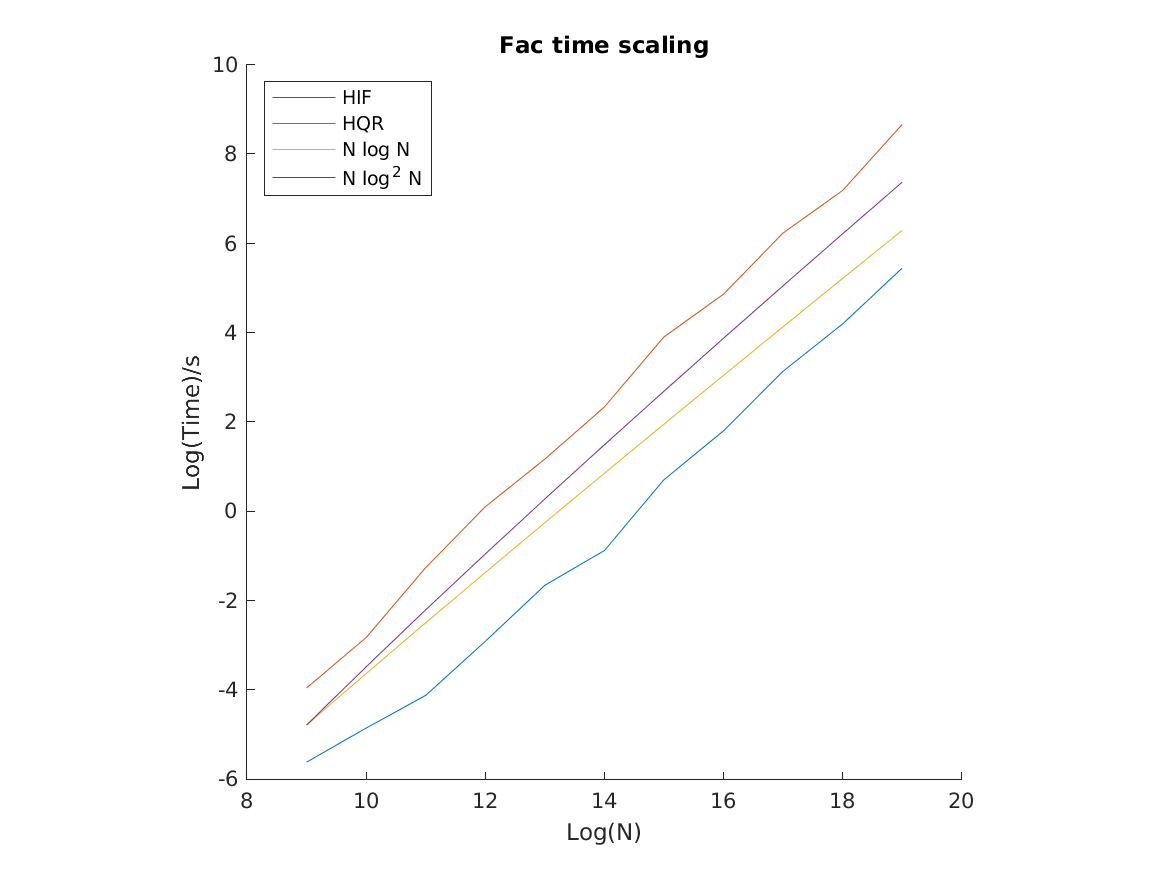
\includegraphics[height=2.7in]{../../scaling/fio/factime_fun_FIO.png}&
      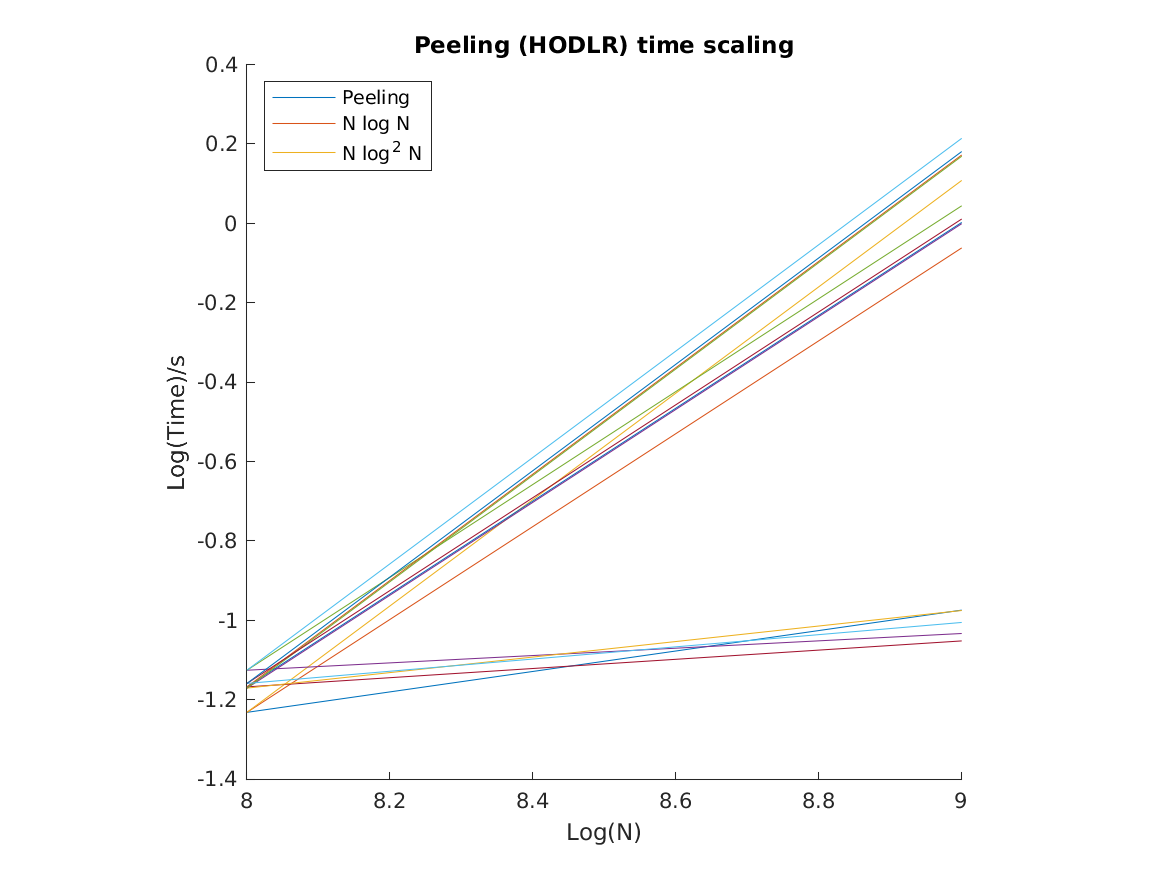
\includegraphics[height=2.7in]{../../scaling/fio/hodlrtime_fun_FIO.png}\\
      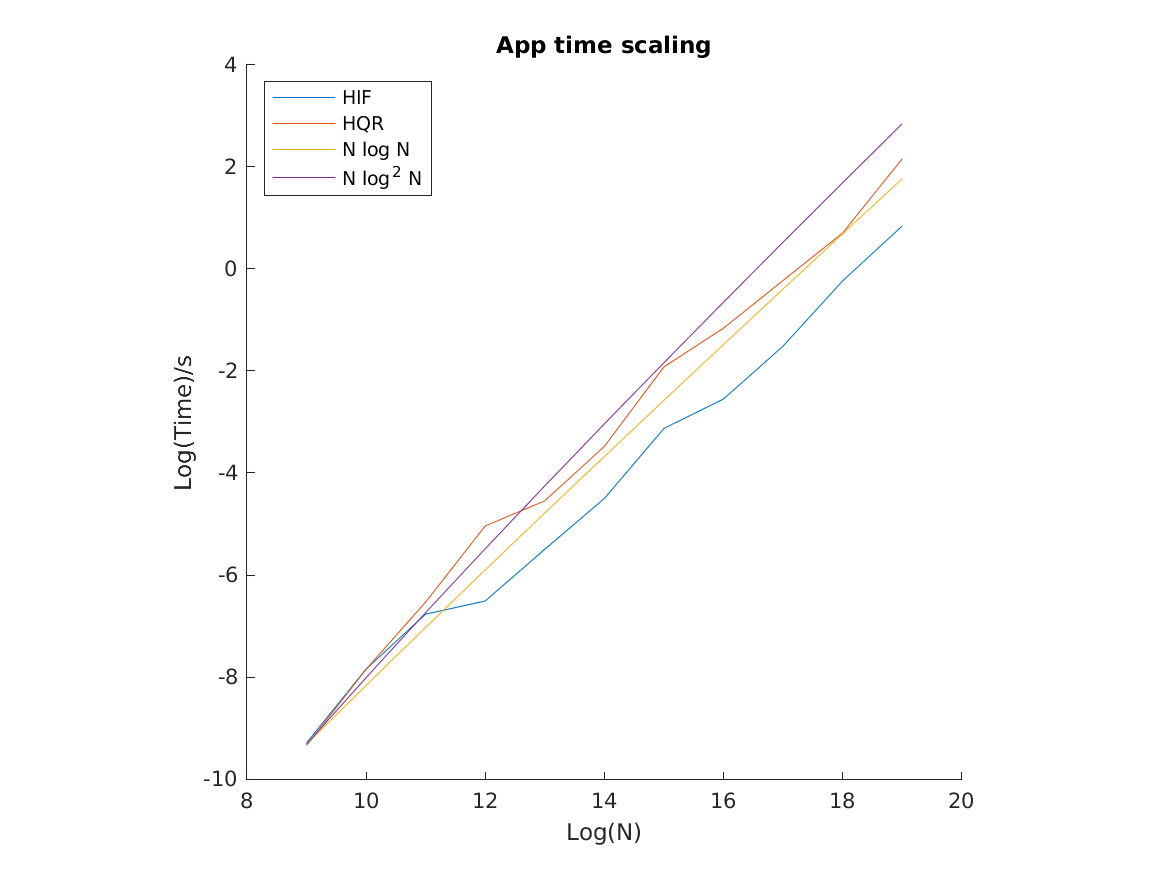
\includegraphics[height=2.7in]{../../scaling/fio/apptime_fun_FIO.png}&   
      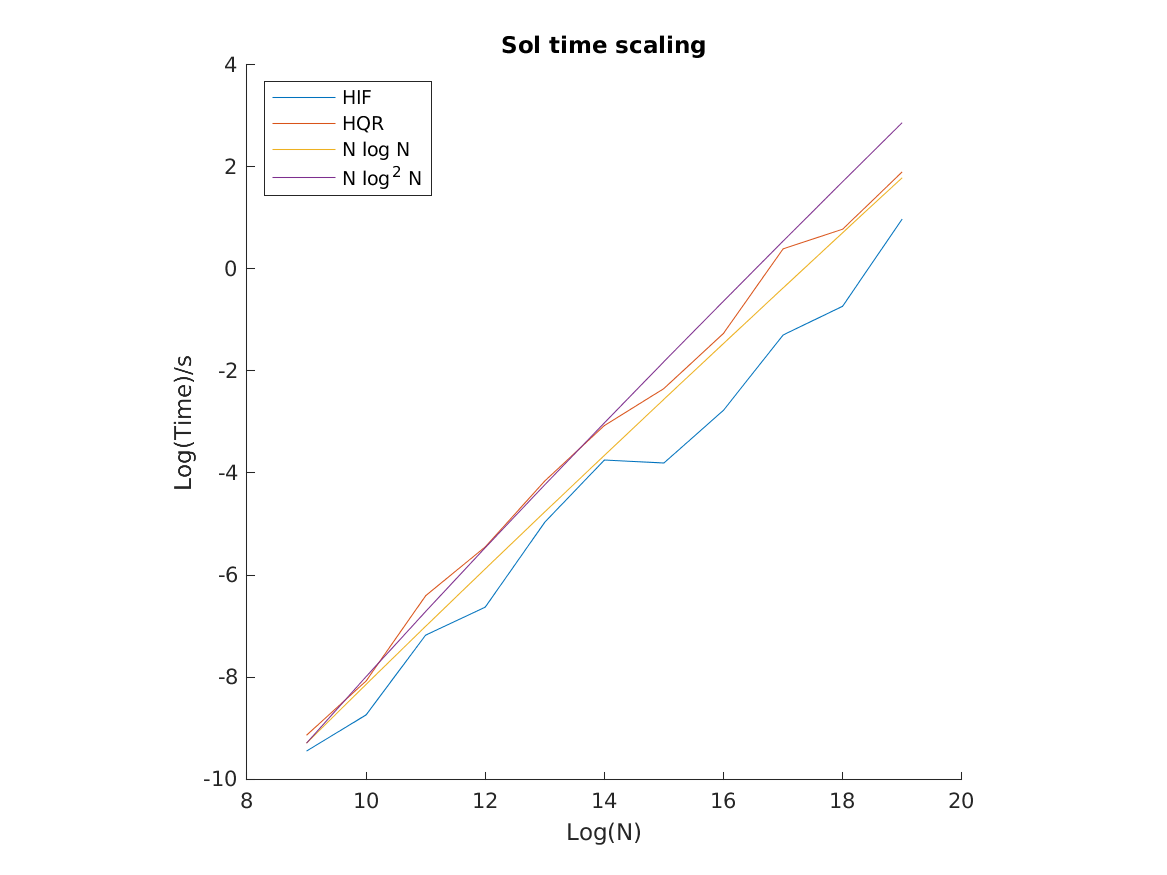
\includegraphics[height=2.7in]{../../scaling/fio/soltime_fun_FIO.png}
    \end{tabular}
  \end{center}
\caption{The upper left, upper right, lower left, and lower right plot the time scaling of HIF/HQR factorization, peeling algorithm, application of HIF/HQR factorization, and backward application of HIF/HQR factorization, respectively. }
\label{fig}
\end{figure}


\begin{table}[!htbp]
\centering
\begin{tabular}{|c|c|c|c|c|c|c|}
\hline
N & cond &Kernel 1 & Kernel 2 & Kernel 3 & Kernel 4 & Kernel 5 \\ 
\hline
$2^{8}$ & $A$ & 1.0660e+02 & 3.4571e+02 & 5.8246e+02 & 2.6794e+02 & 1.6771e+03\\
~ & $A^{*}A$ & 1.1364e+04 & 1.1952e+05 & 3.3926e+05 & 7.1790e+04 & 2.8128e+06\\
\hline
$2^{9}$ & $A$ & 1.1372e+02 & 6.7118e+02 & 3.7644e+02 & 1.6732e+02 & 3.0517e+03\\
~ & $A^{*}A$ & 1.2932e+04 & 4.5048e+05 & 1.4171e+05 & 2.7995e+04 & 9.3131e+06\\
\hline
$2^{10}$ & $A$ & 1.0870e+02 & 3.9350e+03 & 4.4032e+02 & 1.8616e+02 & 3.3981e+03\\
~ & $A^{*}A$ & 1.1815e+04 & 1.5484e+07 & 1.9388e+05 & 3.4657e+04 & 1.1547e+07\\
\hline
$2^{11}$ & $A$ & 1.1999e+02 & 5.2064e+05 & 4.3108e+02 & 1.9745e+02 & 5.0709e+03\\
~ & $A^{*}A$ & 1.4398e+04 & 2.7107e+11 & 1.8583e+05 & 3.8988e+04 & 2.5714e+07\\
\hline
$2^{12}$ & $A$ & 1.2626e+02 & 1.3755e+10 & 5.5073e+02 & 1.9459e+02 & 3.4614e+03\\
~ & $A^{*}A$ & 1.5943e+04 & 2.9863e+17 & 3.0330e+05 & 3.7866e+04 & 1.1981e+07\\



\end{tabular}

\caption{Condition numbers of all kernels}
\label{cond}
\end{table}




\begin{table}[!htbp]
\centering
\begin{tabular}{|c|c|c|c|c|c|c|c|c|c|c|c|c|c|c|}
\hline
\multicolumn{1}{c|}{} & \multicolumn{1}{c|}{$\hat{K} \approx K$} & \multicolumn{2}{c|}{$HODLR$} & \multicolumn{1}{c|}{} &\multicolumn{4}{c|}{HIF} & \multicolumn{4}{c|}{HQR} & \multicolumn{2}{c|}{CG} \\
\hline
N & $e_{a}$ & $e_{h}$ & $r_{h}$ & $\epsilon$ & $e_{f}$ & $e_{s}$ & $n_{i}$ & $e$ & $e_{f}$  & $e_{s}$ & $n_{i}$ & $e$ &  $n_{i}$ & $e$ \\ 
\hline
$2^{8}$ & 1e-15 & 2e-09 & 33 & 1e-4 & 8e-06 & 4e-05 & 4 & 8e-14 & 4e-05 & 3e-04 & 5 & 3e-13 & 120 & 3e-07\\
~ & ~ & 2e-09 & 33 & 1e-6 & 9e-08 & 7e-07 & 3 & 8e-14 & 4e-07 & 2e-06 & 3 & 1e-13 & 120 & 3e-07\\
~ & ~ & 2e-10 & 36 & 1e-8 & 1e-09 & 3e-08 & 2 & 1e-13 & 3e-09 & 4e-08 & 2 & 7e-14 & 120 & 3e-07\\
~ & ~ & 1e-13 & 46 & 1e-12 & 1e-13 & 2e-12 & 2 & 7e-14 & 2e-13 & 3e-12 & 2 & 2e-14 & 120 & 3e-07\\
\hline
$2^{9}$ & 1e-15 & 1e-09 & 38 & 1e-4 & 1e-05 & 1e-04 & 4 & 9e-14 & 7e-05 & 2e-04 & 6 & 3e-12 & 120 & 1e-05\\
~ & ~ & 1e-09 & 38 & 1e-6 & 1e-07 & 1e-06 & 3 & 8e-14 & 6e-07 & 2e-06 & 3 & 1e-13 & 120 & 1e-05\\
~ & ~ & 2e-10 & 42 & 1e-8 & 1e-09 & 2e-08 & 2 & 1e-13 & 6e-09 & 1e-08 & 2 & 8e-14 & 120 & 6e-05\\
~ & ~ & 2e-13 & 52 & 1e-12 & 3e-13 & 2e-12 & 2 & 7e-14 & 4e-13 & 2e-12 & 2 & 1e-13 & 119 & 5e-04\\
\hline
$2^{10}$ & 1e-15 & 2e-09 & 43 & 1e-4 & 1e-05 & 9e-05 & 4 & 5e-13 & 9e-05 & 2e-04 & 5 & 5e-13 & 103 & 2e-02\\
~ & ~ & 2e-09 & 43 & 1e-6 & 1e-07 & 2e-06 & 3 & 6e-14 & 7e-07 & 2e-06 & 3 & 7e-14 & 103 & 2e-02\\
~ & ~ & 2e-10 & 48 & 1e-8 & 1e-09 & 3e-08 & 2 & 6e-14 & 5e-09 & 2e-08 & 2 & 1e-13 & 102 & 1e-02\\
~ & ~ & 7e-13 & 60 & 1e-12 & 9e-13 & 1e-11 & 2 & 1e-13 & 1e-12 & 1e-11 & 2 & 8e-14 & 95 & 2e-02\\
\hline
$2^{11}$ & 3e-11 & 2e-09 & 48 & 1e-4 & 2e-05 & 2e-04 & 5 & 6e-14 & 8e-05 & 2e-04 & 5 & 4e-12 & 109 & 1e-02\\
~ & ~ & 2e-09 & 47 & 1e-6 & 2e-07 & 1e-06 & 3 & 2e-14 & 8e-07 & 2e-06 & 3 & 1e-13 & 90 & 2e-02\\
~ & ~ & 2e-10 & 53 & 1e-8 & 2e-09 & 3e-08 & 2 & 2e-13 & 9e-09 & 2e-08 & 2 & 3e-13 & 120 & 3e-03\\
~ & ~ & 3e-12 & 64 & 1e-12 & 3e-12 & 2e-11 & 2 & 3e-14 & 4e-12 & 2e-11 & 2 & 5e-14 & 120 & 8e-03\\
\hline
$2^{12}$ & 3e-11 & 2e-09 & 52 & 1e-4 & 2e-05 & 2e-04 & 5 & 5e-14 & 9e-05 & 2e-04 & 5 & 9e-13 & 120 & 7e-03\\
~ & ~ & 2e-09 & 53 & 1e-6 & 1e-07 & 2e-06 & 3 & 9e-14 & 9e-07 & 2e-06 & 3 & 9e-14 & 120 & 5e-03\\
~ & ~ & 4e-10 & 58 & 1e-8 & 2e-09 & 3e-08 & 2 & 3e-13 & 9e-09 & 2e-08 & 2 & 1e-13 & 120 & 3e-03\\
~ & ~ & 3e-11 & 64 & 1e-12 & 3e-11 & 6e-10 & 2 & 6e-14 & 3e-11 & 6e-10 & 2 & 1e-13 & 120 & 2e-03\\
\hline
$2^{13}$ & 3e-11 & 2e-09 & 58 & 1e-4 & 2e-05 & 2e-04 & 5 & 5e-14 & 9e-05 & 2e-04 & 6 & 9e-12 & 118 & 1e-02\\
~ & ~ & 2e-09 & 58 & 1e-6 & 1e-07 & 4e-06 & 3 & 4e-14 & 1e-06 & 3e-06 & 3 & 8e-13 & 120 & 1e-03\\
~ & ~ & 8e-10 & 63 & 1e-8 & 2e-09 & 3e-08 & 2 & 2e-13 & 1e-08 & 2e-08 & 2 & 2e-14 & 97 & 1e-02\\
~ & ~ & 3e-10 & 64 & 1e-12 & 3e-10 & 1e-09 & 2 & 3e-14 & 3e-10 & 1e-09 & 2 & 5e-14 & 120 & 2e-03\\
\hline
$2^{14}$ & 2e-11 & 2e-09 & 63 & 1e-4 & 3e-05 & 1e-04 & 5 & 5e-14 & 1e-04 & 2e-04 & 6 & 1e-11 & 120 & 3e-03\\
~ & ~ & 3e-09 & 63 & 1e-6 & 1e-07 & 2e-06 & 3 & 3e-14 & 1e-06 & 2e-06 & 3 & 1e-13 & 120 & 5e-03\\
~ & ~ & 3e-09 & 64 & 1e-8 & 4e-09 & 2e-08 & 2 & 4e-13 & 1e-08 & 3e-08 & 2 & 1e-12 & 120 & 3e-03\\
~ & ~ & 1e-09 & 64 & 1e-12 & 1e-09 & 1e-08 & 2 & 1e-13 & 1e-09 & 1e-08 & 2 & 9e-14 & 111 & 2e-03\\
\hline
$2^{15}$ & 5e-11 & 9e-09 & 64 & 1e-4 & 2e-05 & 1e-04 & 5 & 6e-14 & 9e-05 & 2e-04 & 8 & 9e-12 & 120 & 5e-03\\
~ & ~ & 9e-09 & 64 & 1e-6 & 2e-07 & 3e-06 & 3 & 3e-13 & 1e-06 & 3e-06 & 3 & 2e-13 & 120 & 7e-03\\
~ & ~ & 9e-09 & 64 & 1e-8 & 1e-08 & 8e-08 & 2 & 3e-12 & 1e-08 & 7e-08 & 2 & 3e-12 & 120 & 1e-03\\
\hline
$2^{16}$ & 6e-11 & 3e-08 & 64 & 1e-4 & 2e-05 & 1e-04 & 5 & 9e-13 & 1e-04 & 6e-04 & 9 & 2e-11 & 120 & 3e-03\\
~ & ~ & 3e-08 & 64 & 1e-6 & 2e-07 & 4e-06 & 3 & 2e-12 & 1e-06 & 3e-06 & 3 & 3e-12 & 120 & 1e-03\\
~ & ~ & 3e-08 & 64 & 1e-8 & 3e-08 & 2e-07 & 3 & 2e-14 & 4e-08 & 2e-07 & 3 & 2e-14 & 120 & 2e-03\\


\end{tabular}

\caption{Numerical comparison between HIF and HQR. We solve 1D kernel (1) equation by using the approximate inverse $\hat{G}\hat{K}^{*}$ as preconditioners for PCG with tolerance $1e-14$. We also solve the equation by pure CG without any preconditioners and set the maximum iteration number to be 120.}
\label{1d-k1}
\end{table}


\begin{table}[!htbp]
\centering
\begin{tabular}{|c|c|c|c|c|c|c|c|c|c|c|c|c|c|c|}
\hline
\multicolumn{1}{c|}{} & \multicolumn{1}{c|}{$\hat{K} \approx K$} & \multicolumn{2}{c|}{$HODLR$} & \multicolumn{1}{c|}{} &\multicolumn{4}{c|}{HIF} & \multicolumn{4}{c|}{HQR} & \multicolumn{2}{c|}{Pure CG} \\
\hline
N & $e_{a}$ & $e_{h}$ & $r_{h}$ & $\epsilon$ & $e_{f}$ & $e_{s}$ & $n_{i}$ & $e$ & $e_{f}$  & $e_{s}$ & $n_{i}$ & $e$ &  $n_{i}$ & $e$ \\ 
\hline
$2^{8}$ & 1e-15 & 8e-09 & 35 & 1e-4 & 1e-05 & 3e-04 & 4 & 2e-12 & 6e-05 & 3e-04 & 5 & 1e-13 & 107 & 4e-02\\
~ & ~ & 8e-09 & 35 & 1e-6 & 6e-08 & 5e-07 & 3 & 2e-13 & 2e-07 & 2e-06 & 3 & 2e-13 & 107 & 4e-02\\
~ & ~ & 6e-10 & 39 & 1e-8 & 5e-10 & 2e-08 & 2 & 3e-13 & 1e-09 & 2e-08 & 2 & 3e-13 & 107 & 4e-02\\
~ & ~ & 6e-13 & 48 & 1e-12 & 3e-13 & 1e-11 & 2 & 6e-13 & 3e-13 & 1e-11 & 2 & 2e-13 & 107 & 4e-02\\
\hline
$2^{9}$ & 1e-15 & 8e-09 & 42 & 1e-4 & 3e-05 & 2e-04 & 5 & 2e-13 & 1e-04 & 5e-04 & 6 & 3e-13 & 104 & 5e-02\\
~ & ~ & 8e-09 & 42 & 1e-6 & 1e-07 & 1e-06 & 3 & 3e-13 & 3e-07 & 3e-06 & 3 & 4e-13 & 104 & 5e-02\\
~ & ~ & 7e-10 & 46 & 1e-8 & 1e-09 & 9e-08 & 2 & 2e-12 & 3e-09 & 7e-08 & 2 & 1e-12 & 117 & 5e-02\\
~ & ~ & 6e-13 & 59 & 1e-12 & 7e-13 & 2e-11 & 2 & 2e-13 & 7e-13 & 2e-11 & 2 & 3e-13 & 119 & 1e-02\\
\hline
$2^{10}$ & 1e-15 & 8e-09 & 50 & 1e-4 & 4e-05 & 1e-02 & 6 & 5e-11 & 2e-04 & 2e-02 & 5 & 1e+00 & 92 & 5e-02\\
~ & ~ & 8e-09 & 50 & 1e-6 & 4e-07 & 2e-04 & 4 & 1e-11 & 4e-07 & 2e-05 & 4 & 8e-11 & 92 & 5e-02\\
~ & ~ & 8e-10 & 55 & 1e-8 & 2e-09 & 9e-07 & 2 & 1e-10 & 4e-09 & 5e-07 & 2 & 7e-11 & 90 & 4e-02\\
~ & ~ & 1e-11 & 64 & 1e-12 & 1e-11 & 1e-07 & 2 & 2e-11 & 1e-11 & 1e-07 & 2 & 2e-11 & 111 & 6e-02\\
\hline
$2^{11}$ & 2e-11 & 1e-08 & 60 & 1e-4 & 9e-05 & 5e-02 & 13 & 2e-07 & 1e-04 & 4e-02 & 1 & 1e+01 & 107 & 5e-02\\
~ & ~ & 1e-08 & 61 & 1e-6 & 7e-07 & 4e-02 & 7 & 9e-06 & 1e-06 & 3e-02 & 6 & 1e+01 & 104 & 5e-02\\
~ & ~ & 2e-09 & 64 & 1e-8 & 5e-09 & 2e-02 & 5 & 2e-06 & 7e-09 & 2e-02 & 10 & 2e-06 & 118 & 4e-02\\
~ & ~ & 2e-09 & 64 & 1e-12 & 2e-09 & 8e-03 & 6 & 7e-07 & 2e-09 & 8e-03 & 6 & 2e-06 & 118 & 4e-02\\
\hline
$2^{12}$ & 4e-11 & 2e-07 & 64 & 1e-4 & 7e-05 & 5e-02 & 37 & 2e+00 & 2e-04 & 5e-02 & 3 & 3e+01 & 118 & 4e-02\\
~ & ~ & 2e-07 & 64 & 1e-6 & 6e-07 & 4e-02 & 18 & 2e-01 & 1e-06 & 4e-02 & 4 & 1e+00 & 118 & 4e-02\\
~ & ~ & 2e-07 & 64 & 1e-8 & 2e-07 & 3e-02 & 20 & 4e-01 & 2e-07 & 3e-02 & 16 & 1e-01 & 116 & 5e-02\\
~ & ~ & 2e-07 & 64 & 1e-12 & 2e-07 & 5e-02 & 20 & 4e-01 & 2e-07 & 5e-02 & 29 & 4e-01 & 116 & 4e-02\\
\hline
$2^{13}$ & 3e-11 & 3e-05 & 64 & 1e-4 & 1e-04 & 5e-02 & 118 & 8e-01 & 2e-04 & 5e-02 & 2 & 1e+00 & 117 & 5e-02\\
~ & ~ & 2e-05 & 64 & 1e-6 & 2e-05 & 5e-02 & 83 & 4e-01 & 2e-05 & 5e-02 & 23 & 4e-01 & 120 & 5e-02\\
~ & ~ & 3e-05 & 64 & 1e-8 & 3e-05 & 5e-02 & 98 & 3e-01 & 3e-05 & 5e-02 & 77 & 7e-01 & 120 & 5e-02\\
~ & ~ & 3e-05 & 64 & 1e-12 & 3e-05 & 1e-01 & 119 & 7e-01 & 3e-05 & 1e-01 & 118 & 8e-01 & 119 & 5e-02\\
\hline
$2^{14}$ & 5e-11 & 2e-02 & 64 & 1e-4 & 1e-02 & 1e+00 & 120 & 3e-01 & 1e-02 & 1e+00 & 16 & 8e-01 & 119 & 5e-02\\
~ & ~ & 2e-02 & 64 & 1e-6 & 2e-02 & 2e+00 & 119 & 2e-01 & 2e-02 & 2e+00 & 120 & 2e-01 & 118 & 5e-02\\
~ & ~ & 2e-02 & 64 & 1e-8 & 2e-02 & 3e+00 & 120 & 2e-01 & 2e-02 & 3e+00 & 117 & 2e-01 & 119 & 6e-02\\
~ & ~ & 1e-02 & 64 & 1e-12 & 1e-02 & 3e+00 & 120 & 3e-01 & 1e-02 & 3e+00 & 120 & 3e-01 & 113 & 6e-02\\
\hline
$2^{15}$ & 5e-11 & 6e-01 & 64 & 1e-4 & 6e-01 & 3e+01 & 96 & 1e+00 & 6e-01 & 3e+01 & 46 & 1e+00 & 119 & 6e-02\\
~ & ~ & 5e-01 & 64 & 1e-6 & 9e+00 & 3e+01 & 2 & 9e-01 & 4e-01 & 1e+02 & 120 & 1e+00 & 118 & 6e-02\\
~ & ~ & 5e-01 & 64 & 1e-8 & 4e-01 & 2e+01 & 120 & 1e+00 & 4e-01 & 2e+01 & 120 & 1e+00 & 119 & 5e-02\\



\end{tabular}

\caption{Numerical comparison between HIF and HQR. We solve 1D kernel (2) equation by using the approximate inverse $\hat{G}\hat{K}^{*}$ as preconditioners for PCG with tolerance $1e-14$. We also solve the equation by pure CG without any preconditioners and set the maximum iteration number to be 120.}
\label{1d-k2}
\end{table}


\begin{table}[!htbp]
\centering
\begin{tabular}{|c|c|c|c|c|c|c|c|c|c|c|c|c|c|c|}
\hline
\multicolumn{1}{c|}{} & \multicolumn{1}{c|}{$\hat{K} \approx K$} & \multicolumn{2}{c|}{$HODLR$} & \multicolumn{1}{c|}{} &\multicolumn{4}{c|}{HIF} & \multicolumn{4}{c|}{HQR} & \multicolumn{2}{c|}{Pure CG} \\
\hline
N & $e_{a}$ & $e_{h}$ & $r_{h}$ & $\epsilon$ & $e_{f}$ & $e_{s}$ & $n_{i}$ & $e$ & $e_{f}$  & $e_{s}$ & $n_{i}$ & $e$ &  $n_{i}$ & $e$ \\ 
\hline
$2^{8}$ & 9e-16 & 1e-09 & 33 & 1e-4 & 5e-06 & 4e-04 & 5 & 6e-13 & 3e-05 & 1e-03 & 7 & 2e-11 & 101 & 1e-01\\
~ & ~ & 1e-09 & 33 & 1e-6 & 6e-08 & 1e-05 & 3 & 5e-13 & 4e-07 & 9e-06 & 3 & 4e-12 & 101 & 1e-01\\
~ & ~ & 1e-10 & 37 & 1e-8 & 3e-10 & 5e-08 & 2 & 5e-13 & 3e-09 & 1e-07 & 2 & 4e-12 & 101 & 1e-01\\
~ & ~ & 1e-13 & 46 & 1e-12 & 1e-13 & 4e-11 & 2 & 5e-13 & 3e-13 & 4e-11 & 2 & 5e-13 & 101 & 1e-01\\
\hline
$2^{9}$ & 1e-15 & 2e-09 & 37 & 1e-4 & 1e-05 & 2e-03 & 6 & 1e-12 & 5e-05 & 2e-03 & 7 & 6e-11 & 113 & 1e-01\\
~ & ~ & 2e-09 & 37 & 1e-6 & 4e-08 & 5e-06 & 3 & 5e-13 & 5e-07 & 1e-05 & 3 & 1e-12 & 113 & 1e-01\\
~ & ~ & 2e-10 & 40 & 1e-8 & 6e-10 & 1e-07 & 2 & 8e-13 & 6e-09 & 1e-07 & 2 & 5e-12 & 120 & 1e-01\\
~ & ~ & 2e-13 & 53 & 1e-12 & 2e-13 & 7e-11 & 2 & 1e-13 & 5e-13 & 7e-11 & 2 & 8e-13 & 119 & 1e-01\\
\hline
$2^{10}$ & 1e-15 & 2e-09 & 40 & 1e-4 & 7e-06 & 7e-04 & 5 & 4e-11 & 7e-05 & 1e-03 & 10 & 2e-10 & 120 & 1e-01\\
~ & ~ & 2e-09 & 40 & 1e-6 & 4e-08 & 3e-06 & 3 & 4e-13 & 7e-07 & 1e-05 & 3 & 7e-12 & 120 & 1e-01\\
~ & ~ & 2e-10 & 46 & 1e-8 & 6e-10 & 1e-07 & 2 & 9e-13 & 8e-09 & 1e-07 & 2 & 1e-11 & 120 & 1e-01\\
~ & ~ & 7e-13 & 58 & 1e-12 & 7e-13 & 2e-10 & 2 & 1e-13 & 1e-12 & 2e-10 & 2 & 2e-13 & 120 & 1e-01\\
\hline
$2^{11}$ & 3e-11 & 2e-09 & 46 & 1e-4 & 2e-05 & 3e-03 & 6 & 4e-11 & 8e-05 & 2e-03 & 13 & 2e-10 & 119 & 1e-01\\
~ & ~ & 2e-09 & 46 & 1e-6 & 9e-08 & 3e-05 & 3 & 2e-11 & 6e-07 & 1e-05 & 3 & 6e-11 & 119 & 1e-01\\
~ & ~ & 2e-10 & 50 & 1e-8 & 6e-10 & 1e-07 & 2 & 3e-12 & 8e-09 & 1e-07 & 2 & 2e-11 & 120 & 1e-01\\
~ & ~ & 2e-12 & 63 & 1e-12 & 2e-12 & 1e-09 & 2 & 8e-13 & 2e-12 & 1e-09 & 2 & 7e-13 & 120 & 1e-01\\
\hline
$2^{12}$ & 4e-11 & 2e-09 & 51 & 1e-4 & 2e-05 & 2e-03 & 7 & 3e-12 & 8e-05 & 2e-03 & 9 & 1e-10 & 118 & 1e-01\\
~ & ~ & 2e-09 & 51 & 1e-6 & 6e-08 & 2e-05 & 3 & 1e-11 & 9e-07 & 2e-05 & 4 & 4e-13 & 118 & 1e-01\\
~ & ~ & 3e-10 & 57 & 1e-8 & 7e-10 & 2e-07 & 2 & 4e-12 & 1e-08 & 4e-07 & 2 & 3e-11 & 120 & 1e-01\\
~ & ~ & 1e-11 & 64 & 1e-12 & 1e-11 & 5e-09 & 2 & 5e-13 & 1e-11 & 5e-09 & 2 & 4e-13 & 116 & 1e-01\\
\hline
$2^{13}$ & 4e-11 & 2e-09 & 54 & 1e-4 & 2e-05 & 2e-03 & 7 & 1e-11 & 8e-05 & 3e-03 & 104 & 1e-06 & 120 & 1e-01\\
~ & ~ & 2e-09 & 56 & 1e-6 & 6e-08 & 1e-05 & 3 & 1e-11 & 1e-06 & 2e-05 & 4 & 7e-13 & 120 & 1e-01\\
~ & ~ & 5e-10 & 61 & 1e-8 & 9e-10 & 2e-07 & 2 & 9e-12 & 9e-09 & 2e-07 & 2 & 7e-11 & 120 & 1e-01\\
~ & ~ & 7e-11 & 64 & 1e-12 & 6e-11 & 2e-08 & 2 & 2e-13 & 6e-11 & 2e-08 & 2 & 2e-13 & 120 & 1e-01\\
\hline
$2^{14}$ & 2e-11 & 2e-09 & 60 & 1e-4 & 3e-05 & 3e-03 & 8 & 2e-11 & 8e-05 & 2e-03 & 10 & 2e-10 & 120 & 1e-01\\
~ & ~ & 2e-09 & 60 & 1e-6 & 5e-08 & 8e-06 & 3 & 4e-12 & 1e-06 & 2e-05 & 4 & 9e-13 & 120 & 1e-01\\
~ & ~ & 6e-10 & 64 & 1e-8 & 1e-09 & 2e-07 & 2 & 1e-11 & 1e-08 & 2e-07 & 2 & 8e-11 & 120 & 1e-01\\
~ & ~ & 4e-10 & 64 & 1e-12 & 5e-10 & 2e-07 & 2 & 3e-12 & 5e-10 & 2e-07 & 2 & 3e-12 & 120 & 1e-01\\
\hline
$2^{15}$ & 5e-11 & 4e-09 & 64 & 1e-4 & 3e-05 & 3e-03 & 8 & 3e-11 & 9e-05 & 3e-03 & 10 & 2e-10 & 120 & 1e-01\\
~ & ~ & 3e-09 & 64 & 1e-6 & 2e-07 & 2e-05 & 3 & 5e-11 & 1e-06 & 2e-05 & 4 & 9e-13 & 120 & 1e-01\\
~ & ~ & 2e-09 & 64 & 1e-8 & 2e-09 & 1e-06 & 2 & 2e-10 & 1e-08 & 1e-06 & 3 & 4e-13 & 120 & 1e-01\\
\hline
$2^{16}$ & 4e-11 & 7e-09 & 64 & 1e-4 & 3e-05 & 3e-03 & 8 & 1e-10 & 9e-05 & 2e-03 & 16 & 4e-10 & 120 & 1e-01\\
~ & ~ & 8e-09 & 64 & 1e-6 & 2e-07 & 3e-05 & 3 & 1e-10 & 1e-06 & 2e-05 & 4 & 6e-13 & 120 & 1e-01\\
~ & ~ & 9e-09 & 64 & 1e-8 & 8e-09 & 4e-06 & 3 & 5e-13 & 1e-08 & 4e-06 & 3 & 6e-13 & 120 & 1e-01\\


\end{tabular}

\caption{Numerical comparison between HIF and HQR. We solve 1D kernel (3) equation by using the approximate inverse $\hat{G}\hat{K}^{*}$ as preconditioners for PCG with tolerance $1e-14$. We also solve the equation by pure CG without any preconditioners and set the maximum iteration number to be 120.}
\label{1d-k3}
\end{table}


\begin{table}[!htbp]
\centering
\begin{tabular}{|c|c|c|c|c|c|c|c|c|c|c|c|c|c|c|}
\hline
\multicolumn{1}{c|}{} & \multicolumn{1}{c|}{$\hat{K} \approx K$} & \multicolumn{2}{c|}{$HODLR$} & \multicolumn{1}{c|}{} &\multicolumn{4}{c|}{HIF} & \multicolumn{4}{c|}{HQR} & \multicolumn{2}{c|}{Pure CG} \\
\hline
N & $e_{a}$ & $e_{h}$ & $r_{h}$ & $\epsilon$ & $e_{f}$ & $e_{s}$ & $n_{i}$ & $e$ & $e_{f}$  & $e_{s}$ & $n_{i}$ & $e$ &  $n_{i}$ & $e$ \\ 
\hline
$2^{8}$ & 9e-16 & 1e-09 & 34 & 1e-4 & 6e-06 & 9e-05 & 4 & 1e-13 & 2e-05 & 3e-04 & 5 & 4e-13 & 111 & 3e-02\\
~ & ~ & 1e-09 & 34 & 1e-6 & 5e-08 & 7e-07 & 3 & 2e-13 & 3e-07 & 2e-06 & 3 & 1e-13 & 111 & 3e-02\\
~ & ~ & 2e-10 & 36 & 1e-8 & 8e-10 & 8e-08 & 2 & 2e-13 & 5e-09 & 1e-08 & 2 & 1e-13 & 111 & 3e-02\\
~ & ~ & 1e-13 & 46 & 1e-12 & 1e-13 & 3e-12 & 2 & 2e-13 & 3e-13 & 3e-12 & 2 & 1e-13 & 111 & 3e-02\\
\hline
$2^{9}$ & 1e-15 & 2e-09 & 37 & 1e-4 & 4e-06 & 6e-05 & 4 & 2e-13 & 4e-05 & 2e-04 & 5 & 2e-12 & 119 & 2e-02\\
~ & ~ & 2e-09 & 37 & 1e-6 & 6e-08 & 5e-07 & 3 & 1e-13 & 4e-07 & 3e-06 & 3 & 1e-13 & 119 & 2e-02\\
~ & ~ & 1e-10 & 41 & 1e-8 & 5e-10 & 5e-08 & 2 & 3e-14 & 5e-09 & 2e-08 & 2 & 9e-14 & 80 & 6e-02\\
~ & ~ & 2e-13 & 53 & 1e-12 & 2e-13 & 3e-12 & 2 & 6e-14 & 5e-13 & 3e-12 & 2 & 2e-13 & 118 & 2e-02\\
\hline
$2^{10}$ & 1e-15 & 2e-09 & 43 & 1e-4 & 5e-06 & 1e-04 & 4 & 6e-13 & 6e-05 & 4e-04 & 6 & 8e-13 & 120 & 3e-02\\
~ & ~ & 2e-09 & 43 & 1e-6 & 5e-08 & 8e-07 & 3 & 6e-14 & 6e-07 & 2e-06 & 3 & 7e-14 & 120 & 3e-02\\
~ & ~ & 1e-10 & 46 & 1e-8 & 6e-10 & 6e-08 & 2 & 2e-13 & 6e-09 & 2e-08 & 2 & 3e-13 & 120 & 3e-02\\
~ & ~ & 7e-13 & 59 & 1e-12 & 8e-13 & 1e-11 & 2 & 2e-13 & 1e-12 & 2e-11 & 2 & 2e-13 & 120 & 1e-02\\
\hline
$2^{11}$ & 3e-11 & 2e-09 & 47 & 1e-4 & 2e-05 & 2e-04 & 5 & 2e-13 & 8e-05 & 3e-04 & 5 & 4e-12 & 120 & 2e-02\\
~ & ~ & 2e-09 & 47 & 1e-6 & 8e-08 & 7e-06 & 3 & 3e-14 & 7e-07 & 2e-06 & 3 & 2e-12 & 120 & 2e-02\\
~ & ~ & 2e-10 & 52 & 1e-8 & 8e-10 & 2e-08 & 2 & 2e-13 & 7e-09 & 3e-08 & 2 & 4e-13 & 120 & 1e-02\\
~ & ~ & 2e-12 & 64 & 1e-12 & 2e-12 & 6e-11 & 2 & 7e-14 & 2e-12 & 6e-11 & 2 & 1e-13 & 120 & 1e-02\\
\hline
$2^{12}$ & 3e-11 & 2e-09 & 52 & 1e-4 & 2e-05 & 2e-04 & 5 & 5e-14 & 7e-05 & 3e-04 & 5 & 1e-11 & 120 & 1e-02\\
~ & ~ & 2e-09 & 52 & 1e-6 & 6e-08 & 2e-06 & 3 & 1e-13 & 8e-07 & 4e-06 & 3 & 9e-14 & 120 & 1e-02\\
~ & ~ & 3e-10 & 58 & 1e-8 & 1e-09 & 2e-08 & 2 & 4e-13 & 8e-09 & 2e-08 & 2 & 2e-13 & 120 & 1e-02\\
~ & ~ & 1e-11 & 64 & 1e-12 & 1e-11 & 2e-10 & 2 & 8e-14 & 1e-11 & 2e-10 & 2 & 1e-13 & 120 & 1e-02\\
\hline
$2^{13}$ & 4e-11 & 2e-09 & 57 & 1e-4 & 2e-05 & 1e-04 & 5 & 7e-14 & 7e-05 & 3e-04 & 5 & 1e-11 & 120 & 1e-02\\
~ & ~ & 2e-09 & 58 & 1e-6 & 7e-08 & 2e-06 & 3 & 6e-14 & 8e-07 & 2e-06 & 3 & 1e-13 & 120 & 9e-03\\
~ & ~ & 6e-10 & 62 & 1e-8 & 1e-09 & 2e-08 & 2 & 2e-13 & 9e-09 & 4e-08 & 2 & 3e-13 & 120 & 1e-02\\
~ & ~ & 1e-10 & 64 & 1e-12 & 1e-10 & 2e-09 & 2 & 5e-14 & 1e-10 & 2e-09 & 2 & 6e-14 & 120 & 1e-02\\
\hline
$2^{14}$ & 2e-11 & 2e-09 & 62 & 1e-4 & 2e-05 & 2e-04 & 5 & 1e-13 & 8e-05 & 3e-04 & 6 & 2e-12 & 120 & 1e-02\\
~ & ~ & 2e-09 & 62 & 1e-6 & 6e-08 & 6e-06 & 3 & 1e-13 & 9e-07 & 3e-06 & 3 & 3e-13 & 120 & 1e-02\\
~ & ~ & 1e-09 & 64 & 1e-8 & 1e-09 & 2e-08 & 2 & 4e-13 & 9e-09 & 3e-08 & 2 & 1e-13 & 120 & 1e-02\\
~ & ~ & 9e-10 & 64 & 1e-12 & 8e-10 & 1e-08 & 2 & 1e-13 & 8e-10 & 1e-08 & 2 & 1e-13 & 120 & 1e-02\\
\hline
$2^{15}$ & 5e-11 & 4e-09 & 64 & 1e-4 & 2e-05 & 1e-04 & 5 & 6e-13 & 8e-05 & 3e-04 & 6 & 5e-13 & 120 & 7e-03\\
~ & ~ & 5e-09 & 64 & 1e-6 & 2e-07 & 3e-06 & 3 & 6e-13 & 1e-06 & 3e-06 & 3 & 3e-14 & 120 & 9e-03\\
~ & ~ & 4e-09 & 64 & 1e-8 & 4e-09 & 8e-08 & 2 & 4e-12 & 1e-08 & 7e-08 & 2 & 3e-12 & 120 & 1e-02\\
\hline
$2^{16}$ & 5e-11 & 1e-08 & 64 & 1e-4 & 2e-05 & 3e-04 & 5 & 1e-12 & 8e-05 & 3e-04 & 5 & 6e-12 & 120 & 7e-03\\
~ & ~ & 1e-08 & 64 & 1e-6 & 1e-07 & 6e-06 & 3 & 1e-12 & 1e-06 & 3e-06 & 3 & 2e-14 & 120 & 8e-03\\
~ & ~ & 1e-08 & 64 & 1e-8 & 1e-08 & 2e-07 & 3 & 3e-14 & 2e-08 & 2e-07 & 3 & 3e-14 & 120 & 8e-03\\


\end{tabular}

\caption{Numerical comparison between HIF and HQR. We solve 1D kernel (4) equation by using the approximate inverse $\hat{G}\hat{K}^{*}$ as preconditioners for PCG with tolerance $1e-14$. We also solve the equation by pure CG without any preconditioners and set the maximum iteration number to be 120.}
\label{1d-k4}
\end{table}



\begin{table}[!htbp]
\centering
\begin{tabular}{|c|c|c|c|c|c|c|c|c|c|c|c|c|c|c|}
\hline
\multicolumn{1}{c|}{} & \multicolumn{1}{c|}{$\hat{K} \approx K$} & \multicolumn{2}{c|}{$HODLR$} & \multicolumn{1}{c|}{} &\multicolumn{4}{c|}{HIF} & \multicolumn{4}{c|}{HQR} & \multicolumn{2}{c|}{Pure CG} \\
\hline
N & $e_{a}$ & $e_{h}$ & $r_{h}$ & $\epsilon$ & $e_{f}$ & $e_{s}$ & $n_{i}$ & $e$ & $e_{f}$  & $e_{s}$ & $n_{i}$ & $e$ &  $n_{i}$ & $e$ \\ 
\hline
$2^{8}$ & 9e-16 & 2e-05 & 14 & 1e-3 & 1e-04 & 1e-03 & 3 & 2e-06 & 5e-04 & 2e-02 & 186 & 1e-03 & 193 & 2e-02\\
~ & ~ & 1e-06 & 17 & 1e-4 & 1e-05 & 2e-04 & 3 & 2e-08 & 4e-05 & 2e-04 & 3 & 3e-07 & 193 & 2e-02\\
\hline
$2^{8}$ & 8e-16 & 3e-09 & 32 & 1e-4 & 4e-06 & 2e-03 & 5 & 1e-10 & 6e-05 & 7e-03 & 12 & 1e-10 & 119 & 1e-01\\
~ & ~ & 3e-09 & 32 & 1e-6 & 6e-08 & 2e-05 & 3 & 9e-12 & 7e-07 & 3e-05 & 4 & 2e-12 & 119 & 1e-01\\
~ & ~ & 2e-10 & 36 & 1e-8 & 5e-10 & 1e-06 & 2 & 2e-11 & 3e-09 & 1e-06 & 3 & 1e-11 & 119 & 1e-01\\
~ & ~ & 1e-13 & 46 & 1e-12 & 3e-13 & 4e-10 & 2 & 6e-12 & 4e-13 & 4e-10 & 2 & 1e-11 & 119 & 1e-01\\
\hline
$2^{9}$ & 1e-15 & 4e-09 & 37 & 1e-4 & 1e-05 & 6e-03 & 7 & 4e-11 & 1e-04 & 9e-03 & 12 & 6e-10 & 118 & 2e-01\\
~ & ~ & 4e-09 & 37 & 1e-6 & 1e-07 & 4e-05 & 3 & 8e-11 & 7e-07 & 7e-05 & 4 & 5e-12 & 118 & 2e-01\\
~ & ~ & 4e-10 & 41 & 1e-8 & 1e-09 & 1e-06 & 2 & 6e-11 & 7e-09 & 1e-06 & 3 & 3e-12 & 116 & 1e-01\\
~ & ~ & 4e-13 & 54 & 1e-12 & 3e-13 & 7e-10 & 2 & 4e-12 & 5e-13 & 6e-10 & 2 & 2e-12 & 119 & 1e-01\\
\hline
$2^{10}$ & 1e-15 & 3e-09 & 40 & 1e-4 & 1e-05 & 9e-03 & 9 & 1e-10 & 8e-05 & 1e-02 & 44 & 1e-03 & 118 & 2e-01\\
~ & ~ & 3e-09 & 40 & 1e-6 & 1e-07 & 3e-05 & 3 & 8e-11 & 1e-06 & 1e-04 & 4 & 2e-10 & 118 & 2e-01\\
~ & ~ & 3e-10 & 45 & 1e-8 & 8e-10 & 5e-07 & 2 & 4e-11 & 8e-09 & 9e-07 & 3 & 4e-12 & 115 & 1e-01\\
~ & ~ & 8e-13 & 58 & 1e-12 & 7e-13 & 1e-09 & 2 & 4e-12 & 9e-13 & 1e-09 & 2 & 5e-12 & 117 & 2e-01\\
\hline
$2^{11}$ & 3e-11 & 3e-09 & 44 & 1e-4 & 3e-05 & 7e-02 & 14 & 2e-10 & 9e-05 & 4e-02 & 5 & 1e+00 & 117 & 2e-01\\
~ & ~ & 3e-09 & 44 & 1e-6 & 2e-07 & 1e-04 & 4 & 1e-11 & 1e-06 & 3e-04 & 5 & 1e-09 & 117 & 2e-01\\
~ & ~ & 3e-10 & 49 & 1e-8 & 8e-10 & 2e-06 & 2 & 2e-10 & 1e-08 & 5e-06 & 3 & 4e-12 & 119 & 2e-01\\
~ & ~ & 2e-12 & 64 & 1e-12 & 2e-12 & 9e-09 & 2 & 4e-12 & 2e-12 & 8e-09 & 2 & 2e-12 & 118 & 2e-01\\
\hline
$2^{12}$ & 3e-11 & 4e-09 & 49 & 1e-4 & 3e-05 & 4e-02 & 16 & 2e-10 & 1e-04 & 2e-02 & 9 & 2e-01 & 120 & 2e-01\\
~ & ~ & 4e-09 & 47 & 1e-6 & 1e-07 & 4e-04 & 4 & 1e-10 & 1e-06 & 2e-04 & 5 & 2e-10 & 117 & 2e-01\\
~ & ~ & 4e-10 & 55 & 1e-8 & 7e-10 & 1e-06 & 2 & 6e-10 & 1e-08 & 1e-06 & 3 & 1e-11 & 117 & 2e-01\\
~ & ~ & 1e-11 & 64 & 1e-12 & 1e-11 & 4e-08 & 2 & 4e-12 & 1e-11 & 4e-08 & 2 & 4e-12 & 120 & 2e-01\\
\hline
$2^{13}$ & 4e-11 & 4e-09 & 52 & 1e-4 & 4e-05 & 6e-02 & 18 & 7e-10 & 1e-04 & 3e-02 & 5 & 2e+00 & 120 & 2e-01\\
~ & ~ & 4e-09 & 53 & 1e-6 & 8e-08 & 1e-04 & 4 & 1e-10 & 1e-06 & 1e-04 & 5 & 2e-09 & 119 & 2e-01\\
~ & ~ & 5e-10 & 58 & 1e-8 & 1e-09 & 1e-06 & 2 & 3e-10 & 1e-08 & 2e-06 & 3 & 3e-12 & 120 & 2e-01\\
~ & ~ & 4e-11 & 64 & 1e-12 & 4e-11 & 2e-07 & 2 & 9e-12 & 4e-11 & 2e-07 & 2 & 1e-11 & 120 & 2e-01\\
\hline
$2^{14}$ & 3e-11 & 4e-09 & 59 & 1e-4 & 5e-05 & 1e-01 & 46 & 7e-10 & 1e-04 & 2e-02 & 66 & 2e-01 & 117 & 2e-01\\
~ & ~ & 4e-09 & 59 & 1e-6 & 1e-07 & 9e-05 & 4 & 1e-11 & 1e-06 & 3e-04 & 5 & 3e-10 & 118 & 2e-01\\
~ & ~ & 8e-10 & 63 & 1e-8 & 1e-09 & 3e-06 & 2 & 1e-09 & 1e-08 & 3e-06 & 3 & 4e-12 & 120 & 2e-01\\
~ & ~ & 3e-10 & 64 & 1e-12 & 4e-10 & 2e-06 & 2 & 3e-10 & 4e-10 & 2e-06 & 2 & 3e-10 & 120 & 2e-01\\
\hline
$2^{15}$ & 5e-11 & 4e-09 & 61 & 1e-4 & 4e-05 & 1e-01 & 116 & 1e-09 & 1e-04 & 3e-02 & 2 & 4e+00 & 120 & 2e-01\\
~ & ~ & 4e-09 & 61 & 1e-6 & 3e-07 & 9e-05 & 4 & 4e-11 & 1e-06 & 2e-04 & 5 & 6e-10 & 118 & 2e-01\\
~ & ~ & 1e-09 & 64 & 1e-8 & 2e-09 & 8e-06 & 3 & 4e-11 & 1e-08 & 8e-06 & 3 & 1e-10 & 120 & 2e-01\\
\hline
$2^{16}$ & 4e-11 & 5e-09 & 64 & 1e-4 & 5e-05 & 2e-01 & 120 & 5e-03 & 1e-04 & 2e-02 & 18 & 5e-01 & 118 & 2e-01\\
~ & ~ & 6e-09 & 64 & 1e-6 & 3e-07 & 3e-04 & 4 & 7e-10 & 1e-06 & 1e-04 & 5 & 1e-09 & 120 & 2e-01\\
~ & ~ & 3e-09 & 64 & 1e-8 & 4e-09 & 1e-05 & 3 & 9e-11 & 1e-08 & 1e-05 & 3 & 2e-10 & 120 & 2e-01\\



\end{tabular}

\caption{Numerical comparison between HIF and HQR. We solve 1D kernel (5) equation by using the approximate inverse $\hat{G}\hat{K}^{*}$ as preconditioners for PCG with tolerance $1e-14$. We also solve the equation by pure CG without any preconditioners and set the maximum iteration number to be 120.}
\label{1d-k5}
\end{table}



\bibliographystyle{unsrt} 
\bibliography{ref}

\end{document}

